\section{Evolution of PanDA WMS}
\subsection{Brief Introduction to Titan}
While PanDa  currently uses  more than 100,000  cores at well over 100 Grid sites with a  peak performance  of 0.3 petaFLOPS,  next LHC data taking run will  require more resources  than Grid computing can possibly provide. The Worldwide LHC Computing Grid (WLCG) infrastructure will be sufficient for the planned analysis and data processing, but it will be insufficient  for Monte Carlo (MC) production and any extra activities. Additional computing and storage  resources are therefore required.  To alleviate  these challenges, ATLAS is engaged  in an ambitious  program to expand  the current computing model to include  additional  resources such as the opportunistic   use of supercomputers   as well as commercial and academic clouds. In turn this activity drives evolution of the PanDA WMS.

\subsection{Use of Supercomputers with PanDA}
The idea is to extend the ATLAS Computing Model beyond the Grid into the domains of supercomputers. Modern High Performance Computing  (HPC) involves  a very large number of worker nodes  connected  through a  high-speed   network. The worker nodes can have  multicore CPUs that can be augmented with massively parallel Graphics Processing Units (GPUs) or other types of coprocessors. On an HPC machine, a  typical job is highly parallel and connected,  where each core calculates  a small part of the problem and coordinates the activity via message passing interface (MPI). While this is different from the HEP computing paradigm, where jobs are independent, it still shares common  features  such as the use of parallelization. It is not a requirement  that HPC machines are able to run any possible task, nor is it relevant how many kinds of job types that can be run. What matters is the total number of cycles that can be offloaded from the Grid. Standard  ATLAS  workflow  can not be easily ported to supercomputers   due  to   several   complications such  as specialized worker  node  setups, no  outbound network connections,  limited memory per node, custom operating systems,  etc. A reorganization  of the standard  workflow is therefore needed.
The most suitable task for HPCs in HEP is event generation. Event generators are mostly computational,  stand-alone code, with few input requirements.  There is no need  to stage-in much data. The event generation  in ATLAS corresponds  to
10-15\% of all jobs on the Grid. A more difficult workload to adapt  for HPCs is detector  simulation. Simulation tasks tend to be tied to the framework of a particular simulation and often require  database access for geometry and relevant run conditions.  However,  there is a  lot to be gained  since simulation  tasks correspond to 2/3 of the Grid capacity.
\subsection{Interfacing PanDA with Titan}
The Titan supercomputer, current number two (number one from November 2012 until June 2013) on the Top 500 list is located at the Oak Ridge Leadership Computing  Facility (OLCF) in Oak Ridge National Laboratory, US. Titan, was the first large-scale system to use  a hybrid architecture that utilizes worker nodes with both AMD 16-core Opteron 6274 CPUs and NVIDIA Tesla K20 GPU accelerators.
Integration with Titan is the current focus for PanDA developers. The project aims to integrate Titan with the PanDA system using an updated PanDA Pilot that runs on the front-end node and submits ATLAS payloads to the worker nodes using the local batch system (PBS) via the SAGA (Simple API for Grid Applications) interface \cite{SAGA}. This solves several complications of  running on HPC worker nodes,  including the lack of connectivity to outside world. The pilot can communicate with the PanDA server from the front-end machine. The interactive front-end  machines and the worker nodes  use  a shared  file system  which makes  it  easy  for the pilot to stage-in  any input files that are required by the payload and stage-out the produced output files after the payload has finished at the end of the job. ATLAS Tier 1 computing  center at Brookhaven National Lab is currently  used for data stage out from Titan but in principle  that can be any Grid site.
1) HPC Backfill: HPC facilities are geared towards  large scale jobs by design. Time allocation on an HPC is competitive and large projects are often preferred. About 10\% of capacity on a  typical HPC machine  is unused  due to mismatches between job sizes and available  resources. The worker nodes sit idle because there are not enough of them or they do not have enough time to handle a large scale computing job. On a machine of the scale of Titan, these 10\% correspond to estimated 300M core hours per year. A system that can occupy those temporarily free nodes with smaller scale tasks would be very valuable. This offers a great possibility for PanDA to harvest the opportunistic resources on Titan and use a similar mechanism on other HPCs. Functionality has been added to the PanDA Pilot to collect information about available unused worker nodes on Titan in real time. This allows PanDA to define precisely size and duration of jobs submitted to Titan according to available free resources. First test of the system were quite successful and show great promise in increasing the resource utilization on Titan.
\begin{figure}
\begin{center}
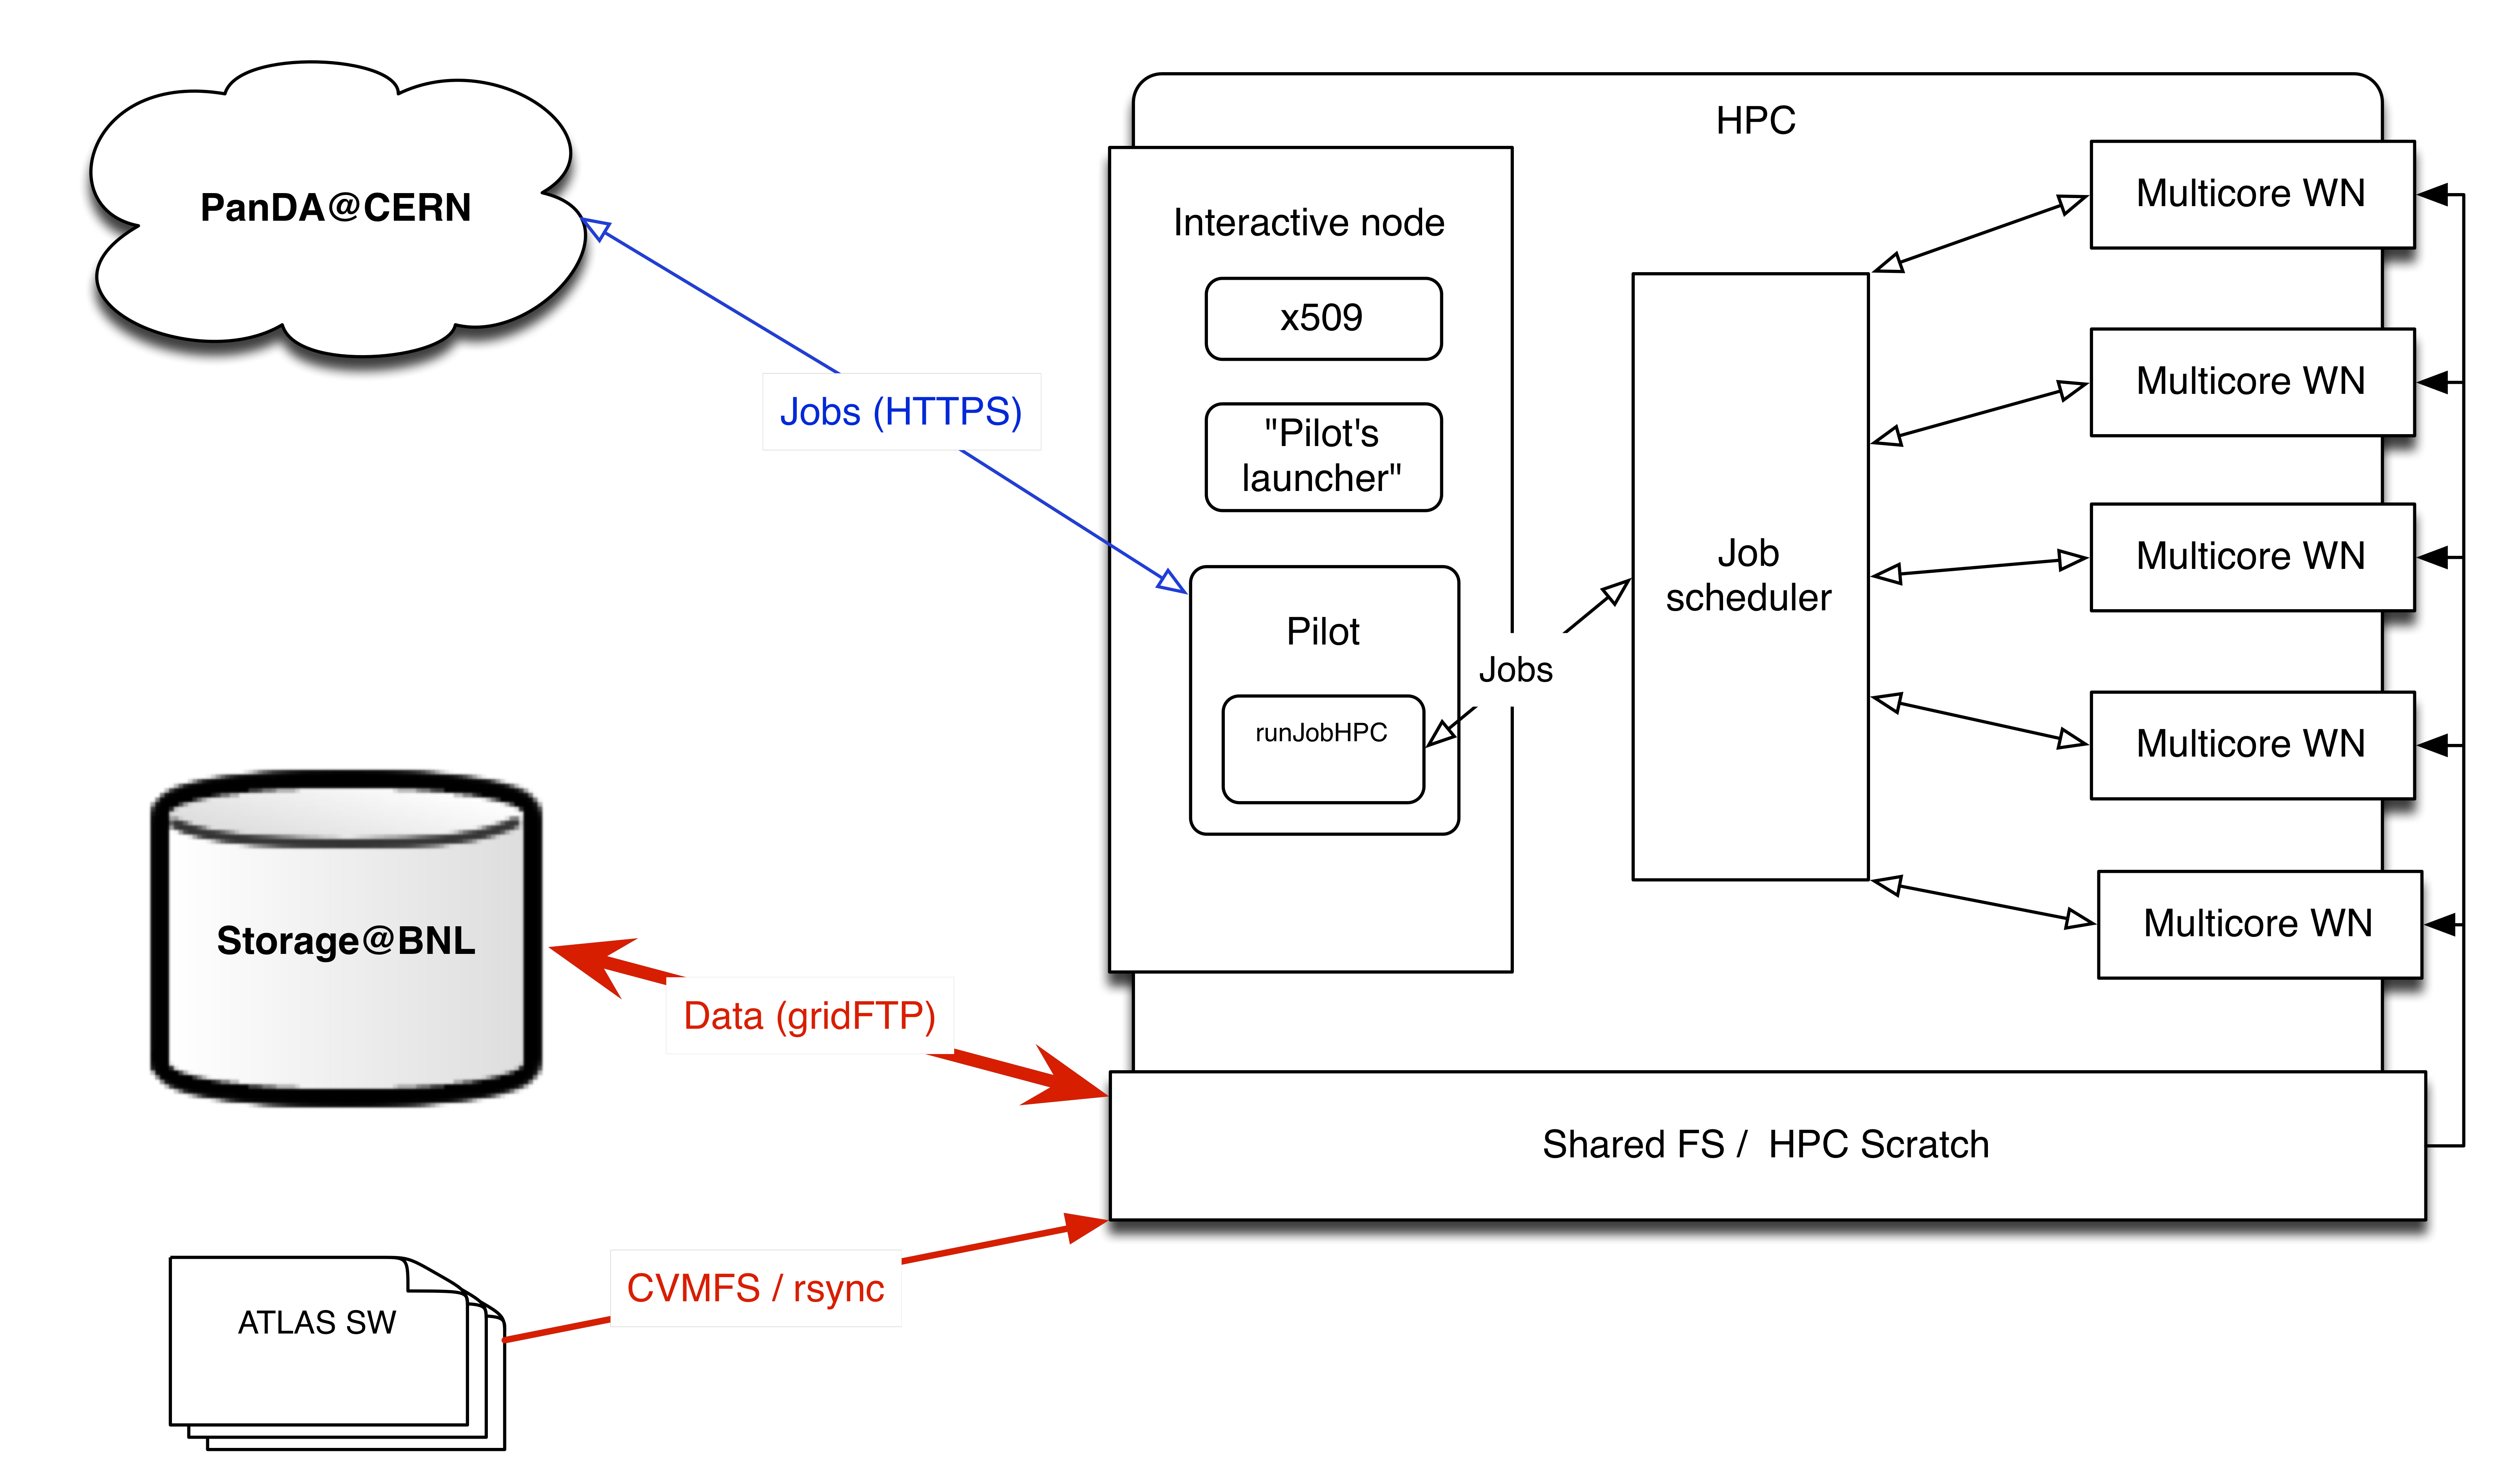
\includegraphics[width=\columnwidth]{figures/PandaInterfaceWithHPC.png}
\caption{Schematic view of the PanDA system\label{fig:interface}}
\end{center}
\end{figure}


